\documentclass[10pt,a4paper]{article}
\usepackage[margin=2cm]{geometry}
\usepackage[T1]{fontenc}
\usepackage{lmodern}
\usepackage{amsmath}
\usepackage{booktabs}
\usepackage{tabularx}
\usepackage{graphicx}
\usepackage{float}
\usepackage[font=small,labelfont=bf]{caption}
\usepackage{enumitem}
\usepackage{xcolor}
\usepackage[hidelinks]{hyperref}

\graphicspath{{../ML_Models/Plots/}{../Gate_Validation/Plots/}{../Test_Circuit/Plots/}}
\setlength{\parindent}{0pt}
\setlength{\parskip}{4pt}
\setlist{nosep,leftmargin=1.2em}
\renewcommand{\arraystretch}{1.12}
\newcommand{\best}[1]{\textbf{#1}}
\newcommand{\pc}{\,\%}

\title{\vspace{-1cm}\textbf{ML Driven PVT Variation Aware Leakage Estimation}\\[2pt]
\large Digital VLSI Design Course Project Report}
\author{\textbf{Team Phasers}\\[2pt]
Rithik Reddy Palla (2024102005) \quad Sale Sangameshwar (2024102017)\\
Regella KRS Kowshik Reddy (2024102053) \quad Gunda Yaswanth Vardhan (2024102012)}
\date{}

\begin{document}
\maketitle
\vspace{-0.8cm}

\section{Setup}

\begin{tabularx}{\linewidth}{@{}lX@{}}
\toprule
Model file & \texttt{45nm\_MGK.pm} (PTM 45 nm metal gate, high k, BSIM4)\\
Nominal VDD & 0.9 V (samples use 0.81 to 0.99 V)\\
Channel length and widths & L = 45 nm, W = 45 to 360 nm (1 to 8 $\times$ Lmin)\\
Test circuit & 3 bit carry lookahead adder (CLA), 42 gates\\
Simulator & ngspice 45.2, batch mode, with \texttt{.options gmin=1e-18 abstol=1e-18 reltol=1e-6 vntol=1e-9} in every netlist\\
Software & Python 3.14, PyTorch 2.15 (CPU), sklearn 1.9, XGBoost 3.4\\
\textbf{Random seed} & \textbf{12175305}, used by every script and notebook (sampling, data split, model training)\\
Metrics & \textbf{Error} = $|{\rm ML}/{\rm SPICE}-1|$ in percent. We report the \textbf{median} error (typical case), the \textbf{95th percentile} error (bad cases) and, for gates and circuit, the \textbf{mean accuracy} = 100\% minus the mean error. Bias is the median signed error.\\
\bottomrule
\end{tabularx}

\section{Data generation}

\textbf{Sampling.} For each of the four cases (NMOS ON, NMOS OFF, PMOS ON, PMOS OFF) every sample draws all inputs independently from the ranges in Table~\ref{tab:ranges}. VDD is drawn first because the drain and source ranges depend on it. Process values are drawn separately for NMOS and PMOS around the nominal values in the model file.

\begin{table}[H]
\centering\small
\begin{tabular}{@{}lll@{}}
\toprule
Input & Range & Notes\\
\midrule
VDD & uniform, 0.9 V $\pm$ 10\% & drawn first\\
Vd, Vs & uniform, 0 to VDD & \\
W & uniform, 45 to 360 nm & L fixed at 45 nm\\
Temperature & uniform, minus 40 to 125 \textdegree C & \\
vth0, toxe, ndep, u0, xj & uniform, nominal $\pm$ 10\% & NMOS nominal vth0 0.3423 V, PMOS $-$0.2312 V\\
Vg, Vb (fixed by case) & ON: Vg = VDD for NMOS, 0 for PMOS & OFF: Vg = 0 for NMOS, VDD for PMOS\\
 & Vb = 0 for NMOS, VDD for PMOS & \\
\bottomrule
\end{tabular}
\caption{Sampling ranges (assignment Section 4).}\label{tab:ranges}
\end{table}

\textbf{Netlists.} Each sample is one DC operating point of one transistor with its own voltage source on drain, gate, source and body. The width and temperature are written into the netlist and the five process values are set with \texttt{altermod}. ngspice prints the four source currents $I_d, I_g, I_s, I_b$. Gate and circuit netlists use the same options line. Inside one corner all NMOS share one process draw and all PMOS share another. Example netlists are in the repository for all four cases, five gates and the CLA.

\textbf{Split.} Random 80/10/10 split of each dataset, \texttt{random\_state} = 12175305. With 20,000 rows this gives 16,000 training, 2,000 validation and 2,000 test rows. The validation set is used for every choice and the test set was used once at the end.

\subsection{Why 10k, then 20k, then 4k extra samples}

\begin{table}[H]
\centering\small
\begin{tabularx}{\linewidth}{@{}lrXX@{}}
\toprule
Stage & Rows per case & Why & Evidence\\
\midrule
First set & 10,000 & The assignment asks for 10,000 samples per case as the initial dataset. This is also the submitted dataset. & Passed the Kirchhoff and trend checks, so the simulation pipeline was trusted before we scaled it.\\
Extended set & 20,000 & The assignment allows more samples if accuracy needs it. A 10k set leaves only 8,000 rows for training. & Learning curve (NMOS\_OFF): training rows 4k, 8k, 12k, 16k give test median 0.33, 0.22, 0.14, 0.13\% and 95th percentile 3.7, 2.4, 1.35, 1.16\%. Going from 8k to 16k training rows nearly halved the error. The curve is flat after 12k, so we stopped at 20k.\\
Gate region rows & +4,000 per model & Gates use transistors in a narrow corner of the input space that uniform sampling almost never visits (details below). & Gate median error fell from 1.42\% to 0.34\% (ON rows) and then to 0.18\% (OFF rows).\\
\bottomrule
\end{tabularx}
\caption{How the training data grew. Rows 1 to 10,000 of the 20k files are exactly the 10k files, with the same seed and the same random stream, so nothing was thrown away.}\label{tab:growth}
\end{table}

\textbf{Why the extra 4,000 rows.} Part B showed that the gate error came from two narrow regions that uniform sampling covers badly.
\begin{itemize}
\item \textbf{ON transistors.} In a gate an ON transistor connects a node to a supply rail, so drain and source are within 20 \textmu V to 1 mV of each other. Only 0.2\% of uniform rows have $|V_{ds}|<1$ mV. There the ON models were 2 to 7\% off on gate and body current. We added 4,000 rows per ON case with Vs near 0 or VDD and Vd right next to it.
\item \textbf{OFF transistors.} With the ON models fixed, the leftover error sat in the channel current of OFF transistors at $|V_{ds}|>0.1$ V. In the gates 52\% of OFF transistors have drain and source at opposite rails, but the 20,000 uniform rows hold only about 8 rows within 2\% of VDD of that corner. We added 4,000 rows per OFF case from these corners.
\end{itemize}
\textbf{Honest note.} These extra rows are single transistor simulations with their own random draws (seeds 12175305 + 1000 to 1003). No gate result was used for training. They are not from the Section 4 distribution and we chose their region after looking at the gate results. They cost the models 0.01 to 0.05 points of median error on the uniform test rows. Rows that fail the data check (no zero current, Kirchhoff residual below $10^{-3}$) were dropped, which leaves 3,915 / 4,000 / 3,997 / 3,911 rows for NMOS ON, NMOS OFF, PMOS ON, PMOS OFF.

\subsection{Data check}

All four 20k datasets pass: columns in the required order, no missing or duplicate rows, no zero currents, every input inside its range, Vg and Vb correct for the case. No row was removed.

\begin{table}[H]
\centering\small
\begin{tabular}{@{}lcccc@{}}
\toprule
 & NMOS ON & NMOS OFF & PMOS ON & PMOS OFF\\
\midrule
Kirchhoff: largest $|I_d+I_g+I_s+I_b|$ / largest current in the row & $1.5\times10^{-4}$ & $8.5\times10^{-6}$ & $9.1\times10^{-6}$ & $2.2\times10^{-4}$\\
Trend checks passed (of 3) & 3 & 3 & 3 & 3\\
\bottomrule
\end{tabular}
\caption{Data check. The Kirchhoff limit is $10^{-3}$. The three trend checks are: OFF current rises with temperature (NMOS $\times$2.9, PMOS $\times$2.6 from minus 40 to 125 \textdegree C), OFF current falls as $|$vth0$|$ rises, and gate current falls as toxe rises. The plots are in \texttt{Data\_Generation/Data\_Check}.}
\end{table}

\section{Models}

\textbf{Inputs and targets.} Every model gets 25 inputs: the 10 raw inputs (vdd, temp, w, vd, vs, vth0, toxe, ndep, u0, xj) plus 15 physics features (voltage differences such as $V_{gs}$ and $V_{ds}$, the sub threshold overdrive divided by the thermal voltage, $1/T$, $\log W$, and $1/t_{ox}$ terms for gate tunnelling). Vg and Vb are not inputs because the case fixes them. The targets are $\log_{10}|I|$ of the four currents, because each current spans 3 to 10 decades. The sign is added afterwards by a simple rule that holds on every row of every dataset. Inputs and targets are standardised with training rows only.

\begin{table}[H]
\centering\small
\begin{tabularx}{\linewidth}{@{}lX@{}}
\toprule
Model type & Main settings\\
\midrule
Random forest & 300 trees, \texttt{max\_features} 0.5\\
XGBoost & learning rate 0.05, depth 4, subsample 0.8, up to 10,000 trees with early stopping\\
Polynomial ridge & degree 1 to 3 and alpha $10^{-4}$ to 100 searched on validation (best: degree 3, alpha 0.01)\\
MLP (MSE) & 25 $\rightarrow$ 128 $\rightarrow$ 64 $\rightarrow$ 32 $\rightarrow$ 16 or 32 $\rightarrow$ 4, SiLU, MSE loss, AdamW (lr 0.01, weight decay $10^{-4}$), batch 256, learning rate halved after 50 flat epochs, early stopping\\
MLP + Kirchhoff loss & as above plus a penalty when the four predicted currents do not sum to zero\\
\best{MLP (Huber loss)} & as MLP, but Huber loss (width 0.002 in standardised units) and 3,000 epochs, keeping the best validation epoch\\
\best{MLP (Huber) + gate region rows} & same recipe, trained on the 16,000 training rows plus 80\% of the 4,000 gate region rows\\
\bottomrule
\end{tabularx}
\caption{The model types compared and their main settings.}
\end{table}

\begin{table}[H]
\centering\scriptsize
\setlength{\tabcolsep}{4pt}
\begin{tabularx}{\linewidth}{@{}lXXXX@{}}
\toprule
Validation set & NMOS ON & NMOS OFF & PMOS ON & PMOS OFF\\
 & \multicolumn{4}{c}{$R^2$ (of $\log|I|$) / median error \% / 95th percentile error \%}\\
\midrule
Random forest & 0.988 / 14.3 / 56.1 & 0.920 / 10.2 / 47.5 & 0.988 / 14.2 / 54.4 & 0.923 / 9.8 / 49.8\\
XGBoost & 0.999 / 3.14 / 14.4 & 0.982 / 3.45 / 20.7 & 0.999 / 2.86 / 12.6 & 0.985 / 3.33 / 19.4\\
Polynomial ridge & 0.996 / 5.79 / 28.0 & 0.869 / 13.7 / 67.0 & 0.997 / 4.46 / 22.1 & 0.868 / 14.6 / 77.3\\
MLP (MSE) & 1.000 / 0.24 / 1.30 & 0.976 / 0.40 / 2.96 & 1.000 / 0.34 / 1.62 & 0.990 / 0.33 / 2.02\\
MLP + Kirchhoff loss & 1.000 / 0.60 / 3.16 & 0.990 / 0.41 / 2.83 & 1.000 / 0.43 / 2.15 & 0.992 / 0.35 / 2.25\\
MLP (Huber loss) & 1.000 / \best{0.10} / \best{0.66} & 0.992 / \best{0.12} / \best{1.02} & 1.000 / \best{0.09} / \best{0.62} & 0.995 / \best{0.12} / \best{0.86}\\
\midrule
\best{MLP (Huber) + gate rows (final)} & 1.000 / 0.15 / 0.89 & 0.992 / 0.13 / 1.18 & 1.000 / 0.14 / 0.86 & 0.996 / 0.14 / 1.09\\
\bottomrule
\end{tabularx}
\caption{Model comparison on the validation set (2,000 rows per case, averaged over the four currents). Bold is the best value among the first six rows.}\label{tab:compare}
\end{table}

\textbf{Which model was chosen and why.}
\begin{itemize}
\item \textbf{MLP over trees and polynomials.} The MLP is about ten times better in median error in all four cases (for example 0.24\% against 3.14\% for XGBoost on NMOS ON). Tree models predict piecewise constant values, which is too coarse for currents that change smoothly over many decades. The polynomial cannot follow the exponential sub threshold behaviour.
\item \textbf{Huber loss over MSE.} A few rows have a current that almost cancels against another one, so $\log|I|$ dives there and MSE spends its effort on them. The Huber loss limits their weight. It lowered the median 2.3 to 3.7 times and the 95th percentile 2.0 to 2.9 times in all four cases, and it removed the training seed luck (with MSE the NMOS OFF test median moved between 0.35\% and 1.08\% from the seed alone, with Huber every seed gave 0.11 to 0.14\%).
\item \textbf{Kirchhoff loss rejected.} The predictions did follow Kirchhoff's law better, but the median and 95th percentile were worse than the plain MLP for both ON cases and no better with Huber.
\item \textbf{Gate region rows kept for the final models.} On uniform validation rows the median is 0.01 to 0.05 points worse, but inside gates the error is much smaller (Section 5).
\end{itemize}

\textbf{How training happened.} Each final model was trained for 3,000 epochs with AdamW and a learning rate that starts at 0.01 and is halved after 50 epochs without validation improvement. Two training seeds (12175305 and 12175306) were run per case and the one with the lower validation error was kept. The saved model is the epoch with the lowest validation loss. The network has 14,260 parameters. One run takes about 5 to 25 minutes on a CPU. We also retrained the Huber MLP with four seeds on a cluster to check stability, and no seed was clearly better.

\begin{table}[H]
\centering\small
\begin{tabular}{@{}lcccc@{}}
\toprule
Test set (2,000 rows) & NMOS ON & NMOS OFF & PMOS ON & PMOS OFF\\
\midrule
$R^2$ (of $\log|I|$) & 0.9997 & 0.9887 & 0.9997 & 0.9959\\
Median error & 0.15\% & 0.14\% & 0.14\% & 0.14\%\\
95th percentile error & 0.88\% & 1.30\% & 0.79\% & 1.15\%\\
\bottomrule
\end{tabular}
\caption{Final transistor models on the test set, averaged over $I_d, I_g, I_s, I_b$. The four model files are in \texttt{ML\_Models/Saved\_Models}.}\label{tab:final}
\end{table}

\begin{figure}[H]
\centering
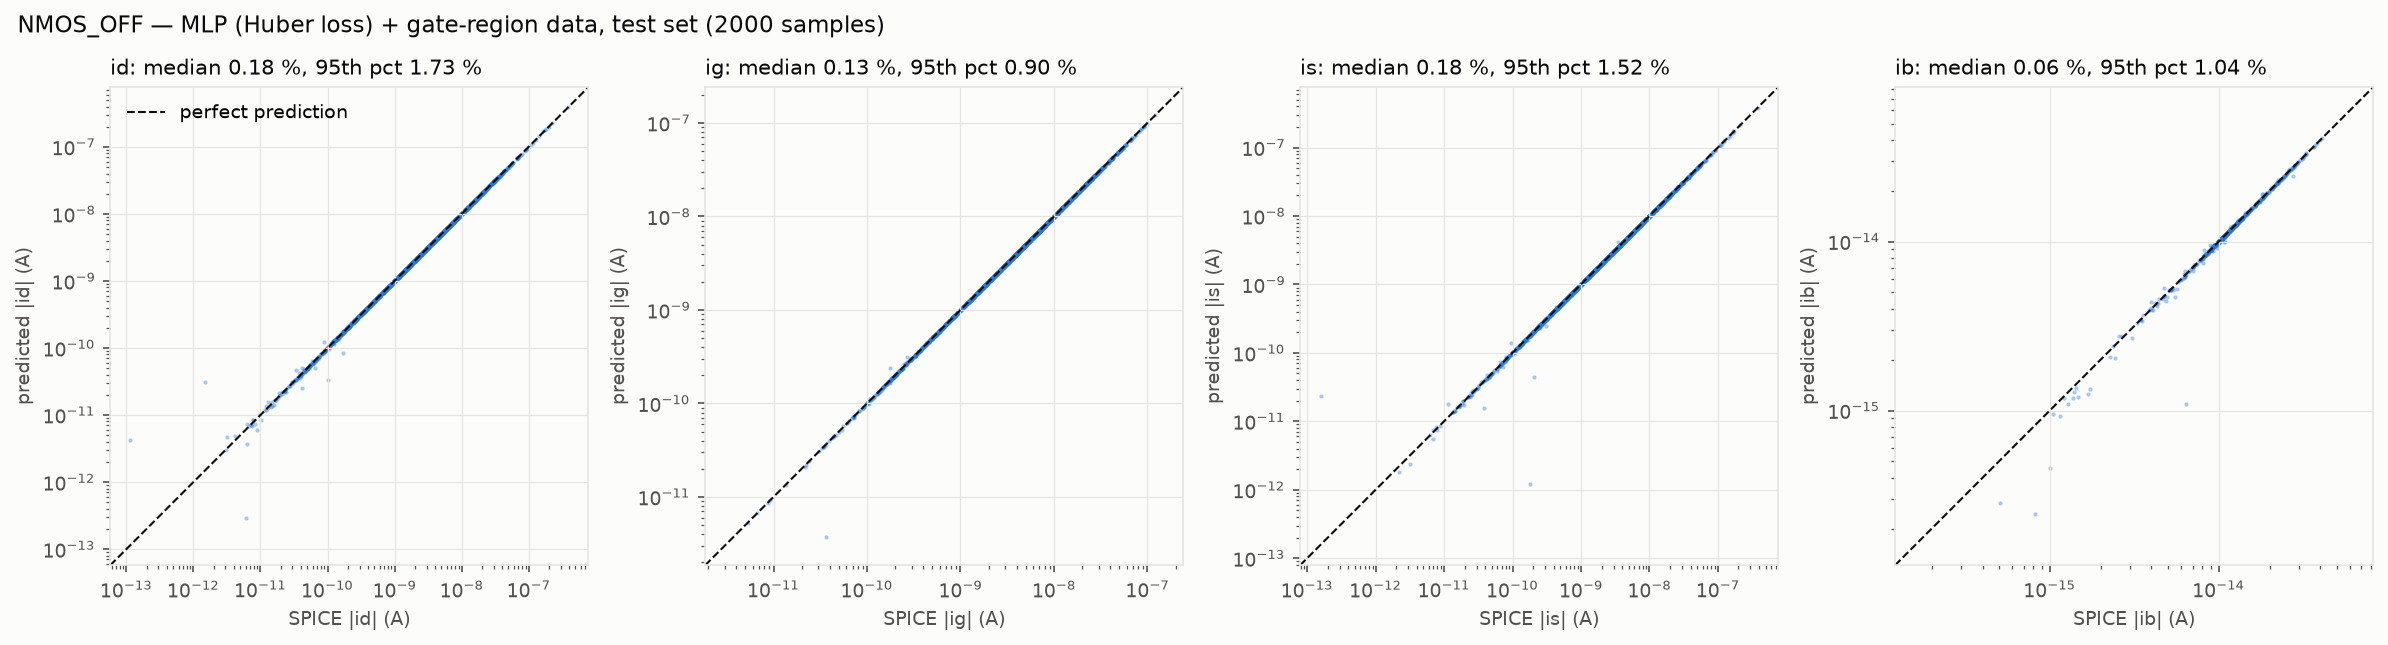
\includegraphics[width=\linewidth]{parity_NMOS_OFF.png}
\caption{Predicted against SPICE current for NMOS OFF on the test set (log axes). This is the hardest case, so we show only this one. The other three cases are tighter and are in \texttt{ML\_Models/Plots}. The few points off the line are the near cancelled currents discussed in Section 7.}
\end{figure}

\section{Gate results}

For each gate and input pattern we simulated 200 corners in SPICE (3,600 points in total, for evaluation only). The ML side takes the internal node and output voltages from SPICE to get each transistor's terminal voltages, picks the ON or OFF model from the gate voltage, and sums the currents drawn from VDD (and from inputs at logic 1). Sizing (L = 45 nm): INV Wn/Wp = 90/180 nm, NAND2 180/180 nm, NOR2 90/360 nm, and AND2 and OR2 are NAND2 or NOR2 plus an INV, simulated as one netlist.

One step needs explaining. The channel current of an ON transistor is solved from Kirchhoff's current law at the internal nodes instead of being read from the model. Inside a gate its $|V_{ds}|$ is only about 0.1 mV and the current is set by the OFF transistors, so a model cannot resolve it. All other currents come from the models.

\begin{table}[H]
\centering\small
\begin{tabular}{@{}llrrrrrr@{}}
\toprule
Gate & Input & SPICE median (A) & ML median (A) & Bias \% & Median err \% & 95th pct err \% & Mean acc \%\\
\midrule
INV & 0 & 6.67e$-$8 & 6.66e$-$8 & 0.04 & 0.20 & 0.79 & 99.72\\
INV & 1 & 8.16e$-$8 & 8.15e$-$8 & $-$0.05 & 0.16 & 0.61 & 99.79\\
NAND2 & 00 & 9.28e$-$8 & 9.29e$-$8 & 0.01 & 0.22 & 0.70 & 99.74\\
NAND2 & 01 & 1.36e$-$7 & 1.35e$-$7 & $-$0.09 & 0.17 & 0.64 & 99.77\\
NAND2 & 10 & 7.54e$-$8 & 7.53e$-$8 & $-$0.04 & 0.18 & 0.64 & 99.74\\
NAND2 & 11 & 2.14e$-$7 & 2.13e$-$7 & $-$0.02 & 0.15 & 0.51 & 99.80\\
NOR2 & 00 & 2.10e$-$7 & 2.10e$-$7 & $-$0.16 & \best{0.32} & 0.99 & 99.62\\
NOR2 & 01 & 2.44e$-$7 & 2.44e$-$7 & $-$0.23 & 0.26 & 0.86 & 99.66\\
NOR2 & 10 & 1.14e$-$7 & 1.14e$-$7 & $-$0.05 & 0.17 & 0.88 & 99.71\\
NOR2 & 11 & 7.79e$-$8 & 7.83e$-$8 & 0.03 & 0.22 & \best{1.32} & 99.63\\
AND2 & 00 & 1.98e$-$7 & 1.98e$-$7 & $-$0.05 & 0.14 & 0.55 & 99.81\\
AND2 & 01 & 2.20e$-$7 & 2.20e$-$7 & $-$0.15 & 0.20 & 0.56 & 99.77\\
AND2 & 10 & 1.55e$-$7 & 1.55e$-$7 & $-$0.13 & 0.18 & 0.63 & 99.77\\
AND2 & 11 & 2.79e$-$7 & 2.78e$-$7 & $-$0.01 & \best{0.12} & \best{0.47} & 99.83\\
OR2 & 00 & 3.14e$-$7 & 3.12e$-$7 & $-$0.25 & 0.28 & 0.81 & 99.67\\
OR2 & 01 & 3.12e$-$7 & 3.12e$-$7 & $-$0.20 & 0.22 & 0.73 & 99.72\\
OR2 & 10 & 1.78e$-$7 & 1.78e$-$7 & $-$0.04 & 0.14 & 0.74 & 99.79\\
OR2 & 11 & 1.45e$-$7 & 1.46e$-$7 & 0.01 & 0.14 & 0.84 & 99.77\\
\midrule
\textbf{All} & & 1.55e$-$7 & 1.55e$-$7 & $-$0.07 & 0.18 & 0.75 & 99.74\\
\bottomrule
\end{tabular}
\caption{Gate results, total leakage (VDD source plus inputs at logic 1), 200 corners per row. Bold marks the worst and best median and 95th percentile.}\label{tab:gates}
\end{table}

\textbf{Most and least accurate.} The most accurate cases are AND2 with inputs 11 and 00, and OR2 with 10 and 11 (median 0.12 to 0.14\%). The least accurate are the NOR2 cases (00 has the highest median at 0.32\%, 11 has the highest 95th percentile at 1.32\%) and OR2 00 (0.28\%). Every case has a median error below 0.35\% and a mean accuracy above 99.6\%, so the 99\% target is met for every gate and input.

\begin{figure}[H]
\centering
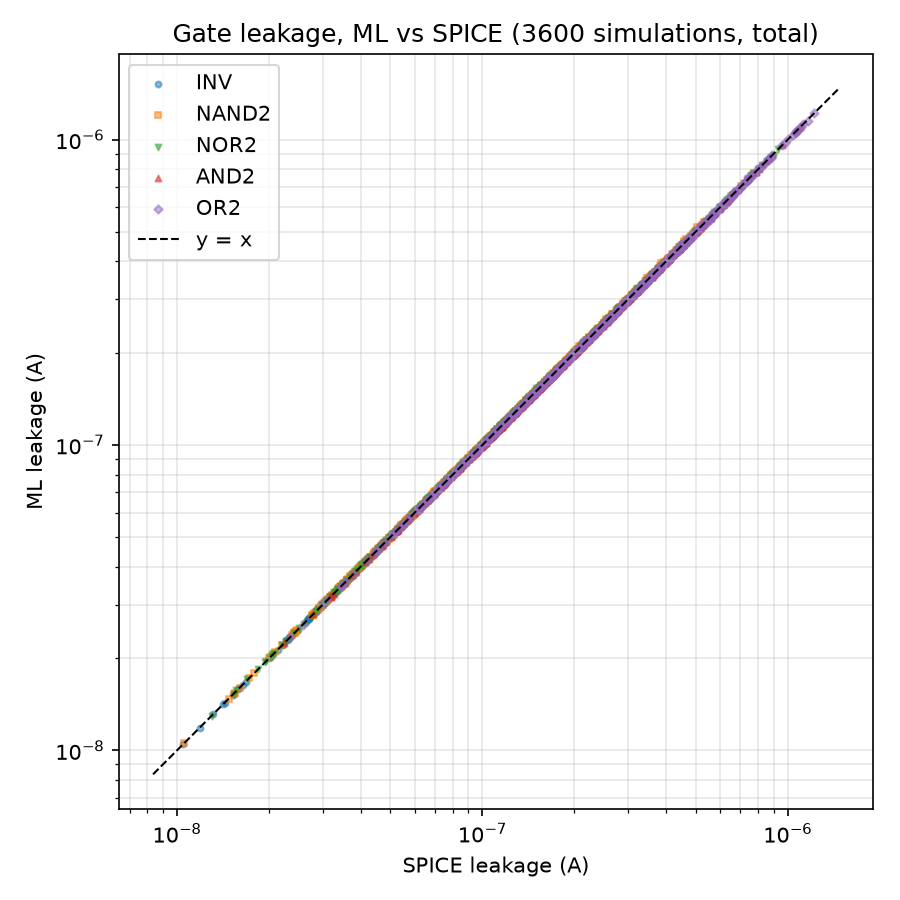
\includegraphics[width=0.45\linewidth]{gate_parity_total.png}\hfill
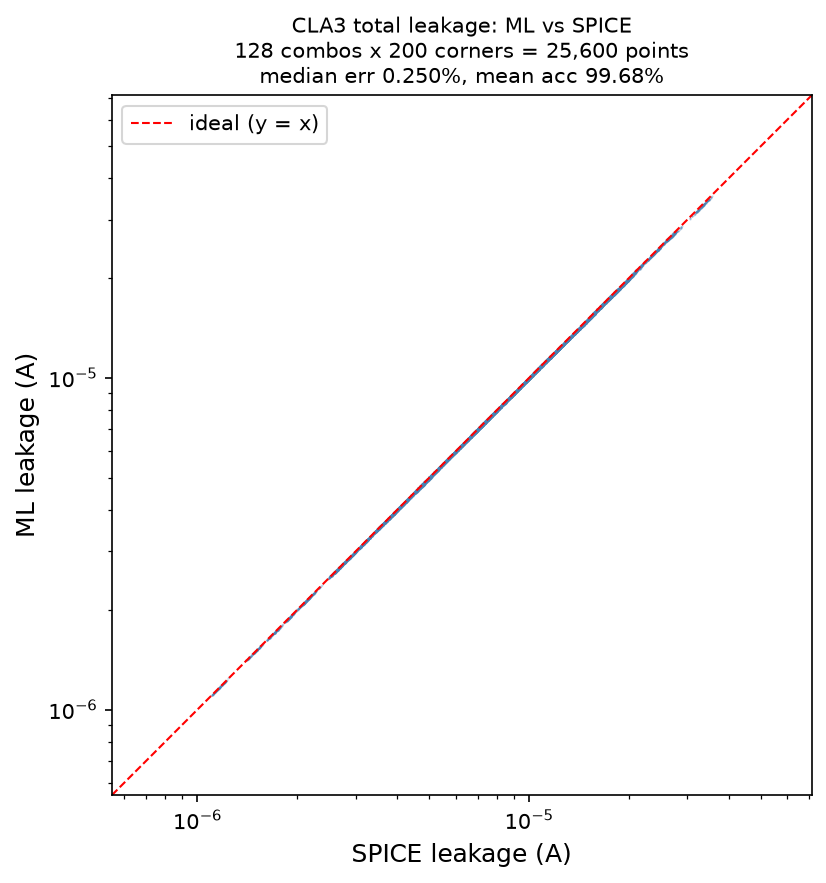
\includegraphics[width=0.45\linewidth]{cla_parity.png}
\caption{ML against SPICE leakage on log axes. Left: all 3,600 gate simulations. Right: the 3 bit CLA, 25,600 points. Points sit on the $y=x$ line over a range of more than one decade.}\label{fig:parity}
\end{figure}

\section{Test circuit results}

The 3 bit CLA has 42 gates (12 AND2, 24 NAND2, 6 OR2, with each XOR built from four NAND2). Every carry is computed directly from the generate and propagate bits and the carry in, so no carry waits for the one before it. We simulated the full transistor netlist for all 128 input combinations at the same 200 corners (25,600 points). For the ML estimate we find the logic value at the input of every gate, look up that gate's ML leakage for the same corner from Part B, and add the 42 values. This assumes every gate input sits at exactly 0 or VDD and ignores loading between gates.

\begin{table}[H]
\centering\small
\begin{tabular}{@{}lrrrrr@{}}
\toprule
 & Points & Bias \% & Median err \% & 95th pct err \% & Mean acc \%\\
\midrule
Gates (Part B) & 3,600 & $-$0.07 & 0.18 & 0.75 & 99.74\\
3 bit CLA (Part C) & 25,600 & $-$0.23 & 0.25 & 0.79 & 99.68\\
\bottomrule
\end{tabular}
\caption{Total leakage, gates against the full circuit. SPICE median leakage of the CLA is 7.56 \textmu A and the ML median is 7.55 \textmu A.}\label{tab:cla}
\end{table}

The circuit is only slightly less accurate than the gates: median error rises from 0.18\% to 0.25\% and the mean accuracy drops from 99.74\% to 99.68\%. The median error stays between 0.19\% and 0.32\% for all 128 input combinations (per combination table in \texttt{Test\_Circuit/Results}), so no input pattern is a problem. The bias grows from $-0.07\%$ to $-0.23\%$. We split this extra error into two parts of similar size. Summing the gates' SPICE leakages against the full circuit SPICE (loading only, no ML) gives a median error of 0.12\% and a bias of $-0.11\%$. Summing the gates' ML leakages against their own SPICE leakages (ML only) gives 0.14\% and $-0.10\%$. The two add up to the 0.25\% and $-0.23\%$ of the circuit. The loading part exists because inside the circuit a gate input is a gate output a few microvolts to millivolts away from the rail, not an ideal source.

\section{Error analysis}

\begin{table}[H]
\centering\small
\begin{tabularx}{\linewidth}{@{}lXX@{}}
\toprule
Where & What we see & Why\\
\midrule
NMOS OFF, $I_d$ and $I_s$ & Median 0.14\%, but mean error 3.07\%. The 5 worst of 2,000 test rows make 82\% of the $I_d$ mean. Without them the mean is 0.6\%. & In an OFF transistor $I_d$ and $I_s$ are the difference of the channel current and the gate and junction leakage. When these nearly cancel (1.2\% of the values) the current is tiny, so a very small absolute error (0.04 to 0.26\% of the row's largest current) becomes a huge percentage. The mean is a poor measure here, which is why we use the median and 95th percentile.\\
OFF models above 85 \textdegree C & Gate error spreads out above about 100 \textdegree C (up to $\pm$3\% at 125 \textdegree C, Figure~\ref{fig:cond}). & OFF currents are largest here and change fastest, and the OFF body current is flat up to about 85 \textdegree C and then rises. We did not isolate the exact cause. The mean accuracy stays high because few points are affected.\\
NOR2 inputs 00 and 11 & Highest gate errors (median 0.32\%, 95th percentile 1.32\%). & Probably because NOR2 uses the widest PMOS (360 nm, near the top of the trained range). With inputs 11 the series OFF PMOS stack leaks little: counting only the VDD source, its leakage is about 10 times below the typical case, so the same absolute error is a larger percentage (median 0.72\%, 95th percentile 4.1\% on that definition).\\
Circuit bias $-0.23\%$ & Slight, steady under prediction. The median error grows with temperature (0.13\% below 0 \textdegree C, 0.53\% above 85 \textdegree C). & About half comes from the ideal rail and no loading assumption and half from the ML gate models. Both slightly underestimate, and leakage is largest when it is hot.\\
\bottomrule
\end{tabularx}
\caption{Where the largest errors occur and the reason.}
\end{table}

\begin{figure}[H]
\centering
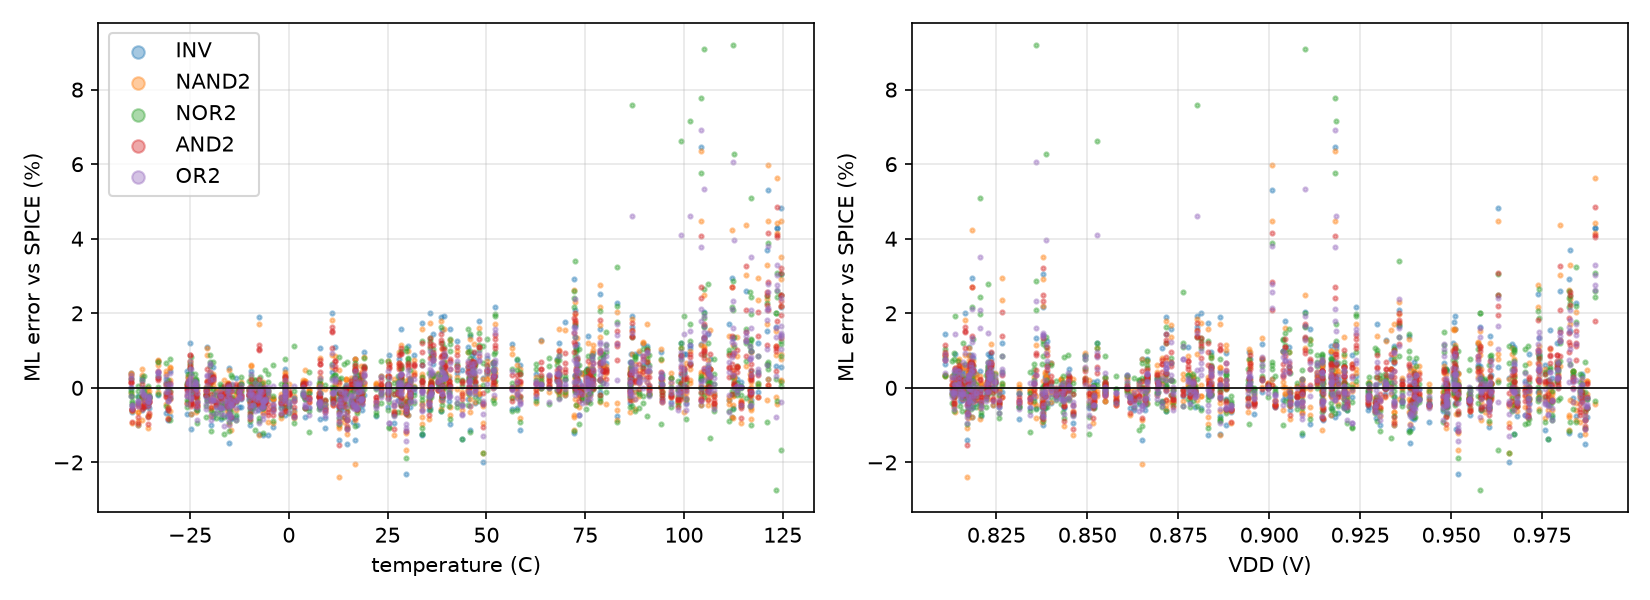
\includegraphics[width=0.85\linewidth]{gate_error_vs_conditions.png}
\caption{Gate error against temperature (left) and VDD (right) for all 3,600 points. The spread grows above 100 \textdegree C and is similar across VDD.}\label{fig:cond}
\end{figure}

\textbf{What fixed the gate error.} Table~\ref{tab:steps} shows each change in order. Adding the Kirchhoff step and the extra rows for ON and OFF transistors brought the median gate error from 4.2\% to 0.18\%. The first version summed the model currents directly and was worst when an ON transistor sat on the VDD net (INV 0, NAND2 00, NOR2 00 and 01, with 8 to 12\% error), because the whole supply current then flows through that ON channel.

\begin{table}[H]
\centering\small
\begin{tabular}{@{}lrrr@{}}
\toprule
Total leakage, gate level & Median err \% & 95th pct err \% & Mean acc \%\\
\midrule
Plain sum of model currents, first version & 4.22 & 13.87 & 94.59\\
+ Kirchhoff for the ON channels & 1.42 & 7.29 & 97.71\\
+ ON models trained with gate region rows & 0.34 & 1.64 & 99.47\\
+ OFF models trained with gate region rows (final) & \best{0.18} & \best{0.75} & \best{99.74}\\
\midrule
For comparison, plain sum with the final models & 6.35 & 36.27 & 89.44\\
\bottomrule
\end{tabular}
\caption{Gate error after each change. The first four rows were recorded when each change was made. The last row is recomputed with the final models. It is high because the ON channel current is deliberately left untrained at tiny $|V_{ds}|$, since Kirchhoff supplies it.}\label{tab:steps}
\end{table}

\section{Limitations and improvements}

\begin{itemize}
\item \textbf{Near cancelled currents.} They limit NMOS OFF accuracy and we could not remove them. A signed log target, a Kirchhoff derived target, bigger networks and an ensemble did not help. \textit{Next:} sample more densely where the sign changes (low source voltage, below 40 \textdegree C) and weight those rows in the loss.
\item \textbf{Temperature range.} OFF models trained only below 85 \textdegree C fail above 105 \textdegree C (median error 14 to 24\%) and widths extrapolate well. The random split hides this because every temperature is in training. Our test conditions stay inside the trained range, so this does not affect the results above. \textit{Next:} widen the temperature coverage if other ranges are needed.
\item \textbf{Extra rows are a design choice.} They improved gates a lot, but they are not from the assignment distribution and the region was picked after seeing gate results. A cleaner method would pick the region from the circuit topology before looking at any result.
\item \textbf{Composition uses SPICE voltages.} As the assignment says, the ML step uses the internal node voltages from SPICE, so errors in predicting those voltages are not tested. \textit{Next:} solve the node voltages from the models.
\item \textbf{Circuit level assumptions.} Gate inputs are taken as ideal rails and loading between gates is ignored, which explains about half of the extra bias (the other half is the ML error of the gates). \textit{Next:} feed real input voltages into the gate models or add a correction for loading.
\item \textbf{Single split and seed.} All numbers use one split and one seed (12175305). The cluster check with four training seeds gave test medians of 0.09 to 0.14\% in every case, so seed noise is small for the final recipe.
\end{itemize}

\end{document}
